%\documentclass[handout]{beamer}
%\documentclass[handout,10pt,slidestop,mathserif]{beamer}
%\usepackage{pgfpages}
%\pgfpagesuselayout{2 on 1}
\documentclass[10pt,slidestop,mathserif,c]{beamer}
\usetheme{Madrid}
\usecolortheme{seahorse}

\usepackage{tabularx}
\usepackage{verbatim}
\usepackage{graphics}
\usepackage{graphicx}
\usepackage{Sweave}
\usepackage{moreverb}
\usepackage{pgf}
\usepackage{tikz}
\usepackage{Sweave}
%\SweaveOpts{prefix.string=figures/}

\newcommand{\putat}[3]{\begin{picture}(0,0)(0,0)\put(#1,#2){#3}\end{picture}}
  
\newenvironment{changemargin}[2]{%
  \begin{list}{}{%
    \setlength{\topsep}{0pt}%
    \setlength{\leftmargin}{#1}%
    \setlength{\rightmargin}{#2}%
    \setlength{\listparindent}{\parindent}%
    \setlength{\itemindent}{\parindent}%
    \setlength{\parsep}{\parskip}%
  }%
  \item[]}{\end{list}}

%% Define a new "leo" style for the package that will use a smaller font.
\makeatletter
\def\url@leostyle{%
  \@ifundefined{selectfont}{\def\UrlFont{\sf}}{\def\UrlFont{\tiny\ttfamily}}}
\makeatother

\title{EPSY 887: Computation Statistics}
\subtitle{Plotting}
\author[Jason Bryer]{Jason Bryer}
\institute[Jason.Bryer.org]{\url{http://github.com/jbryer/CompStats}\\\href{mailto:jason@bryer.org}{jason@bryer.org}}
\date[Feb 18, 2013]{Week 4\\February 18, 2013}

\begin{document}

\AtBeginSection[]
{
   \begin{frame}
       \frametitle{Agenda}
       \tableofcontents[currentsection,currentsubsections]
   \end{frame}
}


\frame{\titlepage}
%\frame{\frametitle{Agenda}\tableofcontents[hideallsubsections]}


\section{ggplot2: A Grammar of Graphics}

\begin{frame}[containsverbatim,fragile]
	\frametitle{ggplot2: A Grammar of Graphics}
	\begin{itemize}
		\item ggplot2 is an R package that provides an alternative framework based upon Wilkinson's (2005) Grammar of Graphics.
		\item ggplot2 is, in general, more flexible for creating "prettier" and complex plots.
		\item Works by creating layers of different types of objects/geometries (i.e. bars, points, lines, polygons, etc.)
		\item ggplot2 has at least three ways of creating plots:
			\begin{enumerate}
				\item \begin{verbatim} qplot \end{verbatim} 
				\item \begin{verbatim} ggplot(...) + geom_XXX(...) + ... \end{verbatim}
				\item \begin{verbatim} ggplot(...) + layer(...) \end{verbatim}
			\end{enumerate}
		We will focus only on the second.
	\end{itemize}
\end{frame}

\begin{frame}[containsverbatim,fragile]
	\frametitle{First Example}
\begin{figure}
\begin{Schunk}
\begin{Sinput}
> data(diamonds)
> p <- ggplot(diamonds, aes(x=carat,y=price,colour=cut)) + 
   	geom_point()
> print(p)
\end{Sinput}
\end{Schunk}
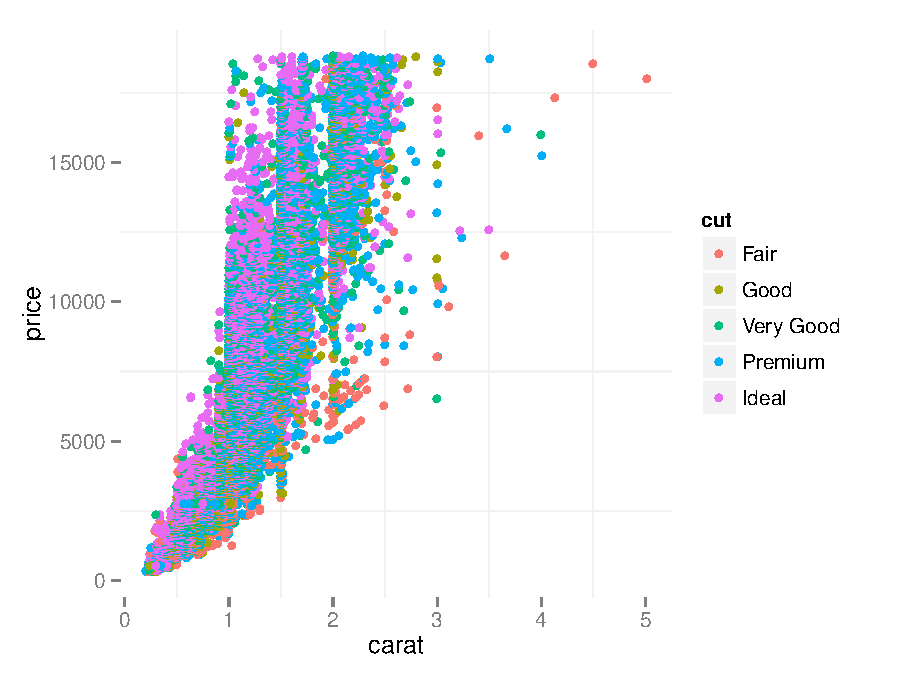
\includegraphics{Slides-ggplot-fig1}
\end{figure}
\end{frame}

\begin{frame}[containsverbatim,fragile]
	\frametitle{First Example}
\begin{figure}
\begin{Schunk}
\begin{Sinput}
> p <- p + facet_wrap(~cut) + 
   	ggtitle("First example")
> print(p)
\end{Sinput}
\end{Schunk}
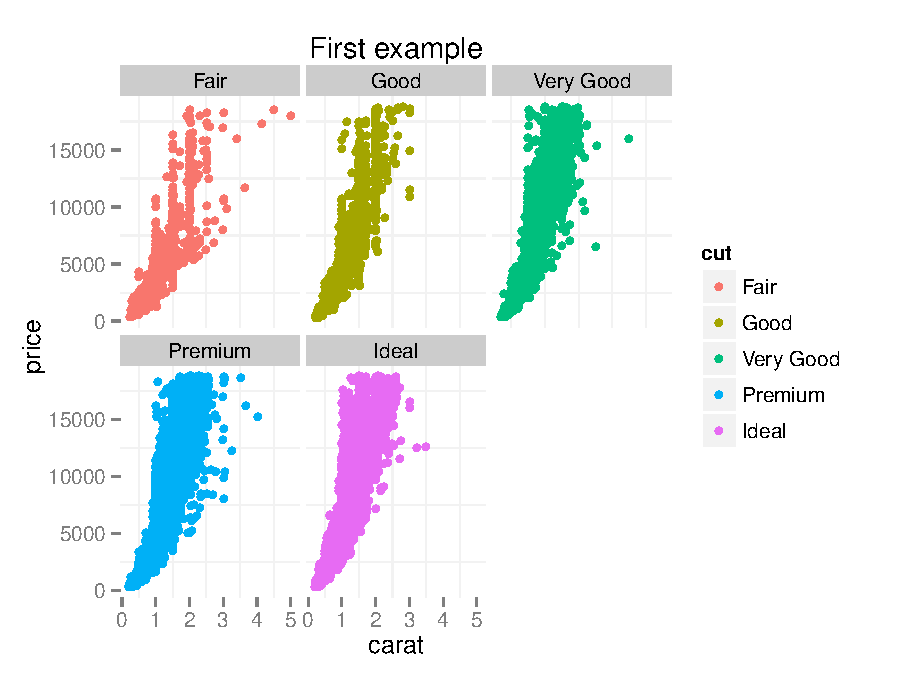
\includegraphics{Slides-ggplot-fig2}
\end{figure}
\end{frame}

\begin{frame}[containsverbatim,fragile]
	\frametitle{Parts of a ggplot2 statement}
	\begin{itemize}
		\item<+-| alert@+> Data \begin{verbatim} ggplot(myDataFrame, aes(x=x, y=y) \end{verbatim}
		\item<+-| alert@+> Layers \begin{verbatim} geom_point(), geom_histogram() \end{verbatim}
		\item<+-| alert@+> Facets \begin{verbatim} facet_wrap(~ cut), facet_grid(~ cut) \end{verbatim}
		\item<+-| alert@+> Scales \begin{verbatim} scale_y_log10() \end{verbatim}
		\item<+-| alert@+> Other options \begin{verbatim} ggtitle("my title"), ylim(c(0, 10000)), xlab("x-axis label") \end{verbatim}
	\end{itemize}
\end{frame}

\begin{frame}[containsverbatim,fragile]
	\frametitle{Lots of geoms}
	\begin{columns}[c]
	\column{1.5in}
\begin{verbatim} 
geom_abline
geom_jitter
geom_area
geom_line
geom_bar	
geom_linerange
geom_bin2d
geom_path 
geom_blank
geom_point 
geom_boxplot
geom_pointrange 
geom_contour
geom_polygon 
geom_crossbar
geom_quantile 
\end{verbatim}
\column{1.5in}
\begin{verbatim}
geom_density
geom_rect 
geom_density2d
geom_ribbon
geom_errorbar
geom_rug
geom_errorbarh
geom_segment 
geom_freqpoly
geom_smooth 
geom_hex
geom_step
geom_histogram
geom_text 
geom_hline
geom_tile
geom_vline
\end{verbatim}
\end{columns}
\end{frame}


\begin{frame}[containsverbatim,fragile]
    \frametitle{Symbols}
\begin{Schunk}
\begin{Sinput}
> p.symbols <- ggplot(data=data.frame(x=c(0:25))) + 
       geom_point(size=10, aes(x=x,y=x,shape=x)) + 
   	facet_wrap(~ x, scales="free") + 
   	xlab("") + ylab("") +
   	scale_shape_identity() +
   	theme(axis.text.x=element_blank(), 
           axis.text.y=element_blank(), 
           axis.ticks=element_blank(), 
           legend.position="none")
\end{Sinput}
\end{Schunk}
\end{frame}

\begin{frame}[containsverbatim,fragile]
	\frametitle{Symbols}
\begin{Schunk}
\begin{Sinput}
> print(p.symbols)
\end{Sinput}
\end{Schunk}
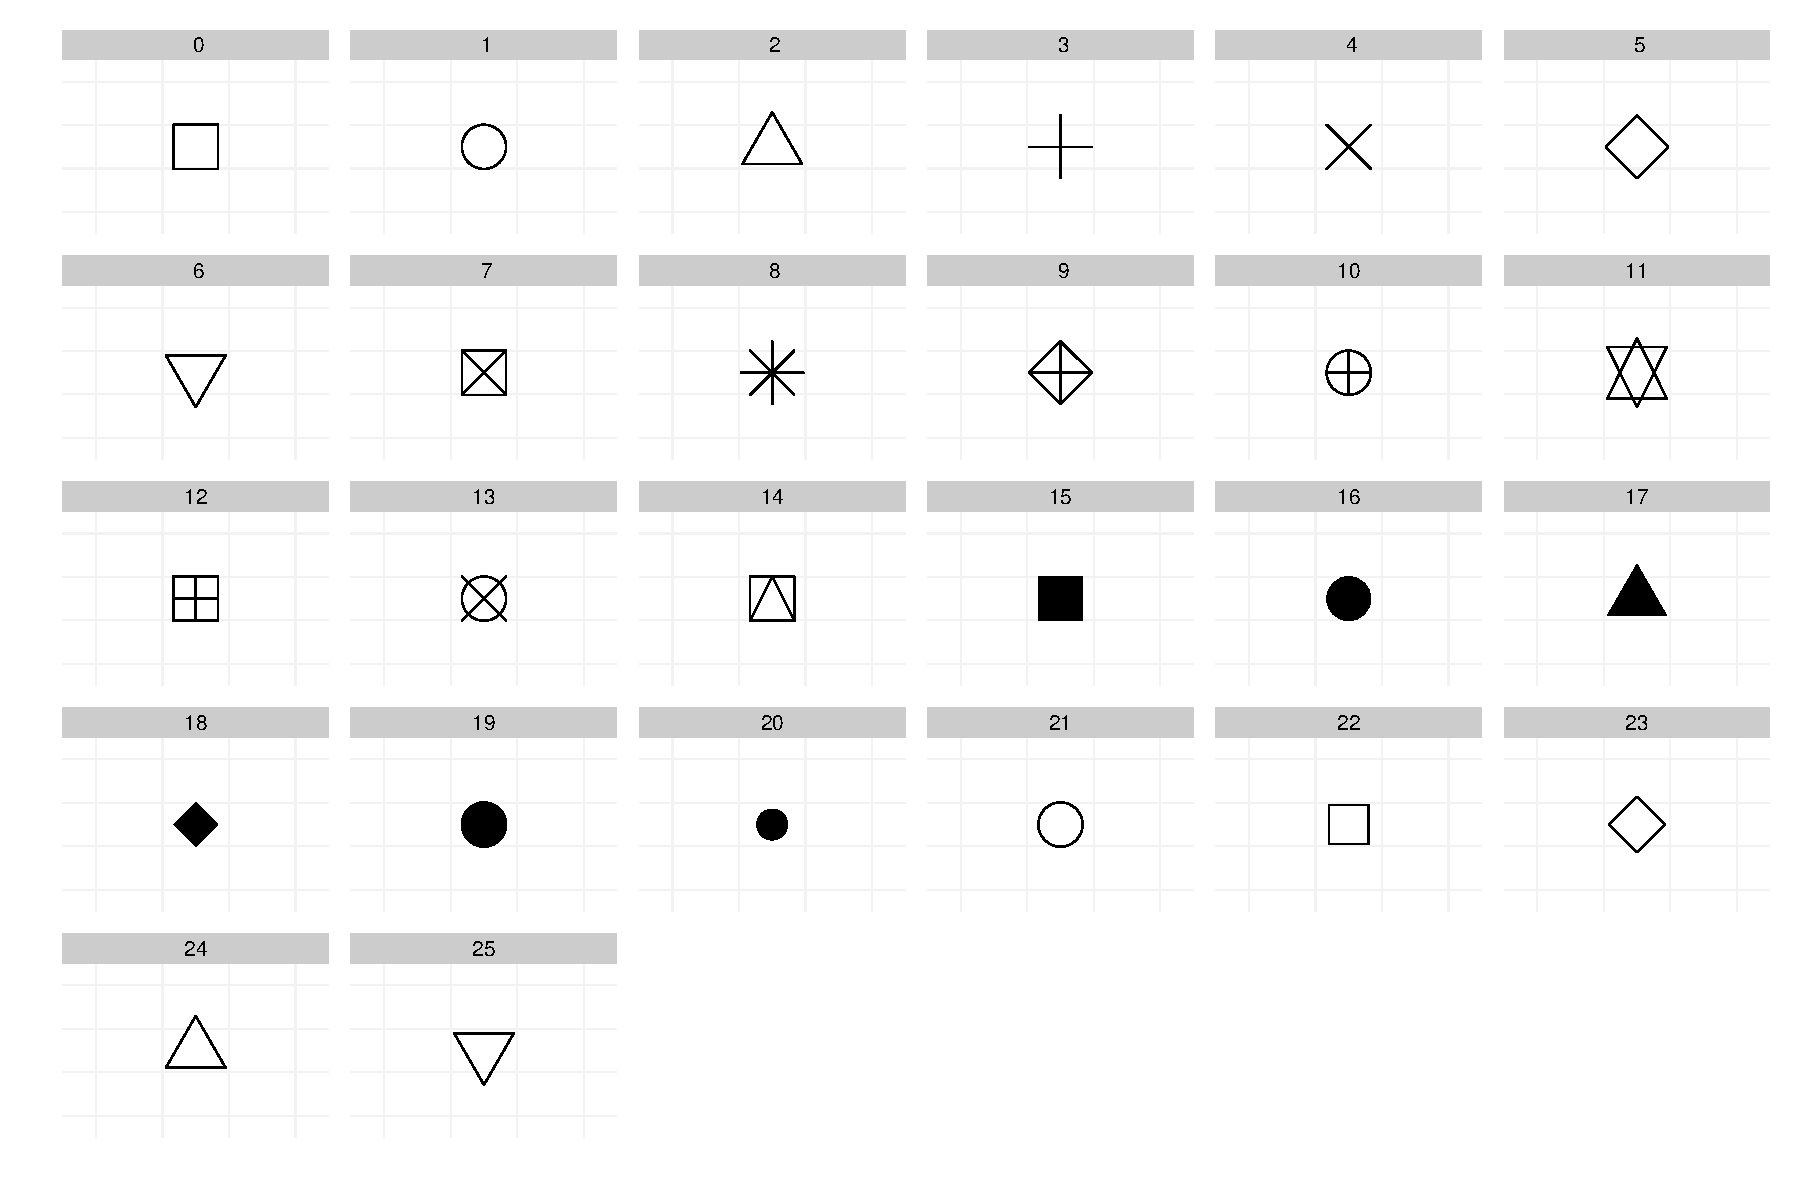
\includegraphics{Slides-symbols}
\end{frame}


\begin{frame}[containsverbatim,fragile]
    \frametitle{Line Types}
\begin{Schunk}
\begin{Sinput}
> p.linetypes <- ggplot(data=data.frame(x=c(1:6))) + 
       geom_hline(size=2, aes(yintercept=x, linetype=x)) +
   	scale_linetype_identity() +
   	xlab(NULL) + ylab(NULL) + xlim(c(0,100)) +
   	theme(axis.text.x=element_blank(), axis.ticks=element_blank(), legend.position="none")
\end{Sinput}
\end{Schunk}
\end{frame}

\begin{frame}[containsverbatim,fragile]
	\frametitle{Line Types}
\begin{Schunk}
\begin{Sinput}
> print(p.linetypes)
\end{Sinput}
\end{Schunk}
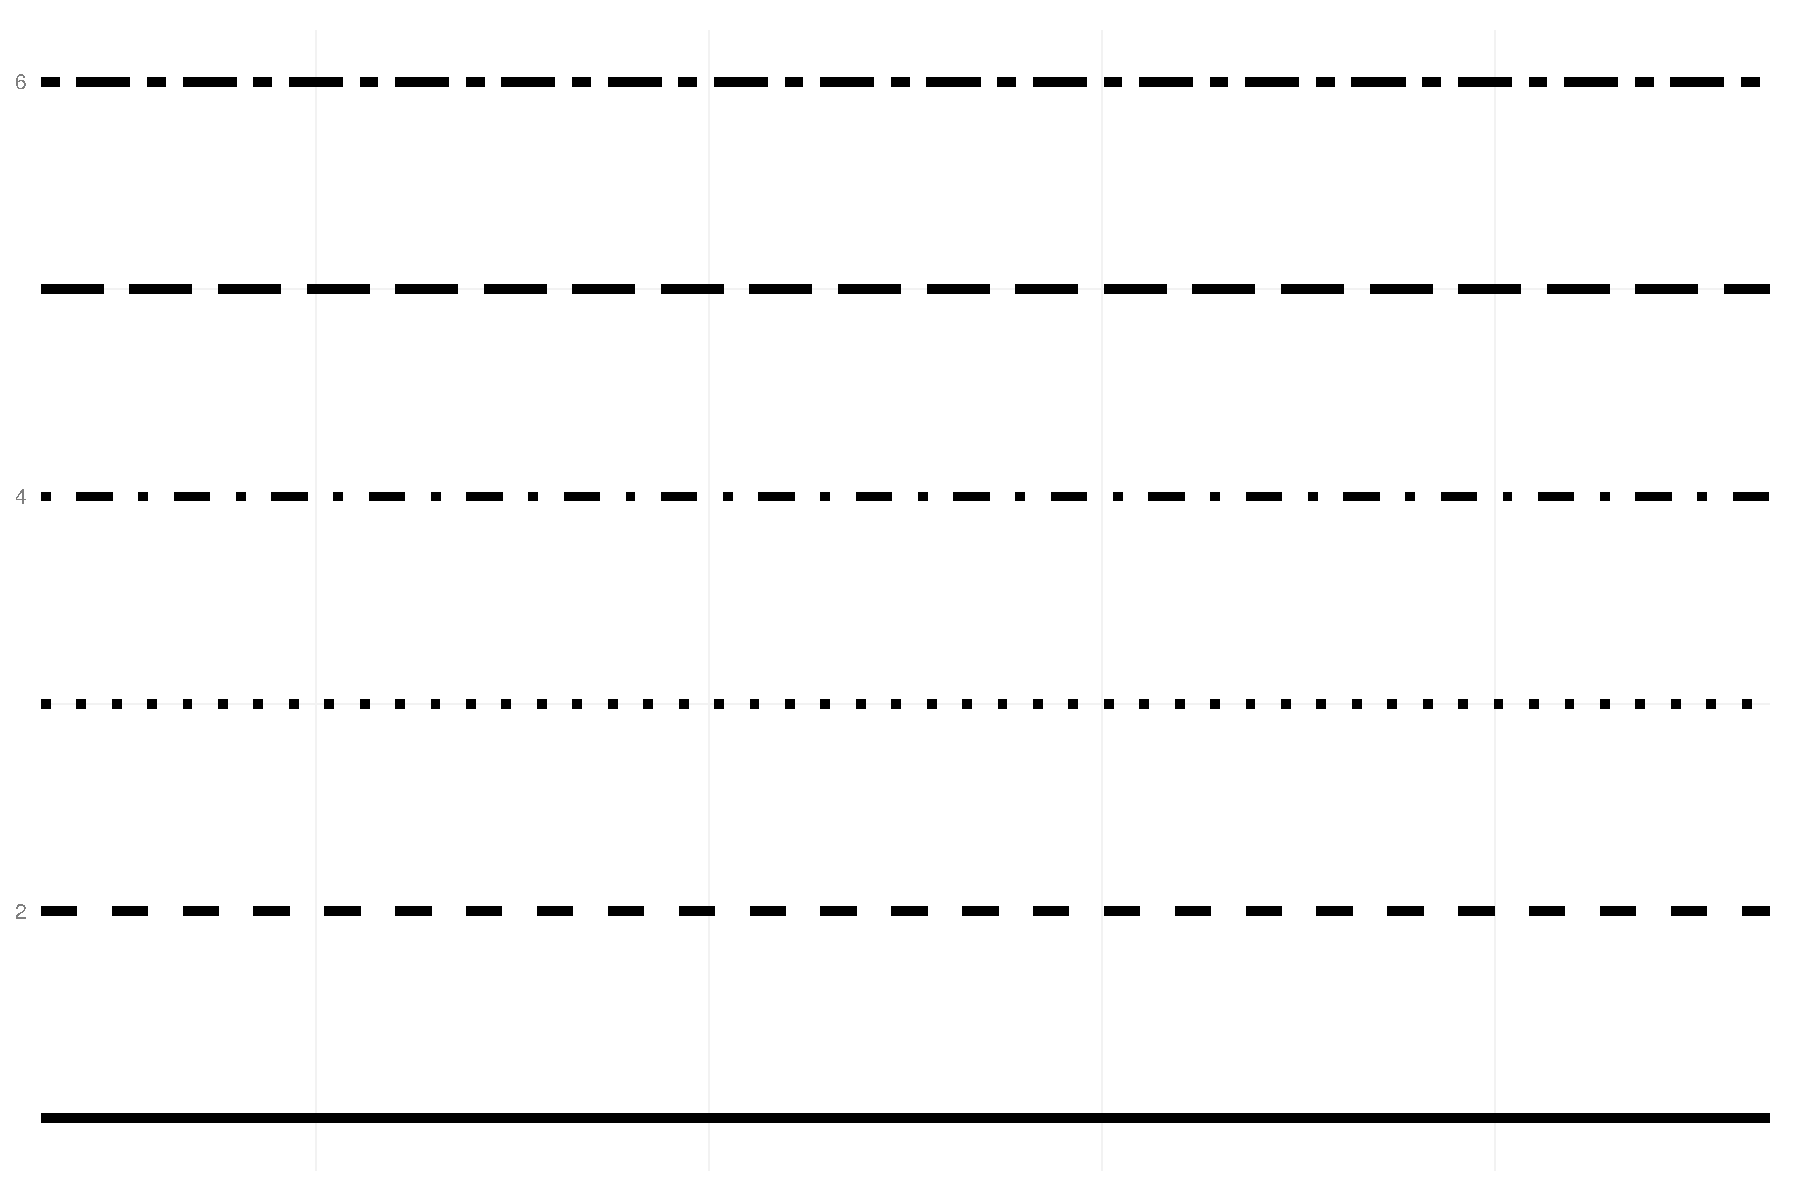
\includegraphics{Slides-linetypes}
\end{frame}

\begin{frame}[containsverbatim,fragile]
    \frametitle{Colors}
\begin{Schunk}
\begin{Sinput}
> getColorHexAndDecimal <- function(color) {
   	if(is.na(color)) {
   		return(NA)
   	} else {
   		c <- col2rgb(color)
   		return(sprintf("#%02X%02X%02X   %3d %3d %3d", 
   		    c[1],c[2],c[3], c[1], c[2], c[3]))
   	}
   }
\end{Sinput}
\end{Schunk}
\end{frame}

\begin{frame}[containsverbatim,fragile]
    \frametitle{Colors}
\begin{Schunk}
\begin{Sinput}
> df = data.frame(x=rep(1:26, 26), y=rep(1:26, each=26))
> df$c = NA
> df[1:length(colors()),"c"] = colors()
> df$n = NA
> df[1:length(colors()),"n"] = 1:length(colors())
> df$r = df$g = df$b = NA
> df[1:length(colors()),c("r","g","b")] = t(col2rgb(colors()))
> df$text = ifelse(apply(df[,c("r","g","b")], 1, sum) > 
       (255*3/2), "black", "white")
> df$hex = lapply(df$c, getColorHexAndDecimal)
> df$hex2 = paste(format(df$n, width=3), 
       format(df$c, width=(max(nchar(df$c))+1)), 
       format(df$hex, width=(max(nchar(df$hex))+1)))
\end{Sinput}
\end{Schunk}
\end{frame}

\begin{frame}[containsverbatim,fragile]
    \frametitle{Colors}
\begin{Schunk}
\begin{Sinput}
> p.colors <- ggplot(df, aes(x=x, y=y, fill=c, label=n)) + 
       geom_tile() + 
   	geom_text(aes(colour=text), size=3) + 
   	scale_fill_identity() +
   	scale_colour_identity() +
   	xlab(NULL) + ylab(NULL) +
   	theme(axis.text.x=element_blank(), 
   	      axis.ticks=element_blank(), 
   		  plot.margin=unit(c(0,0,0,0), "cm"),
   		  axis.text.y=element_blank(), 
   		  axis.ticks=element_blank(), 
   		  legend.position="none")
\end{Sinput}
\end{Schunk}
\end{frame}

\begin{frame}[containsverbatim,fragile]
	\frametitle{Colors}
\begin{Schunk}
\begin{Sinput}
> print(p.colors)
\end{Sinput}
\end{Schunk}
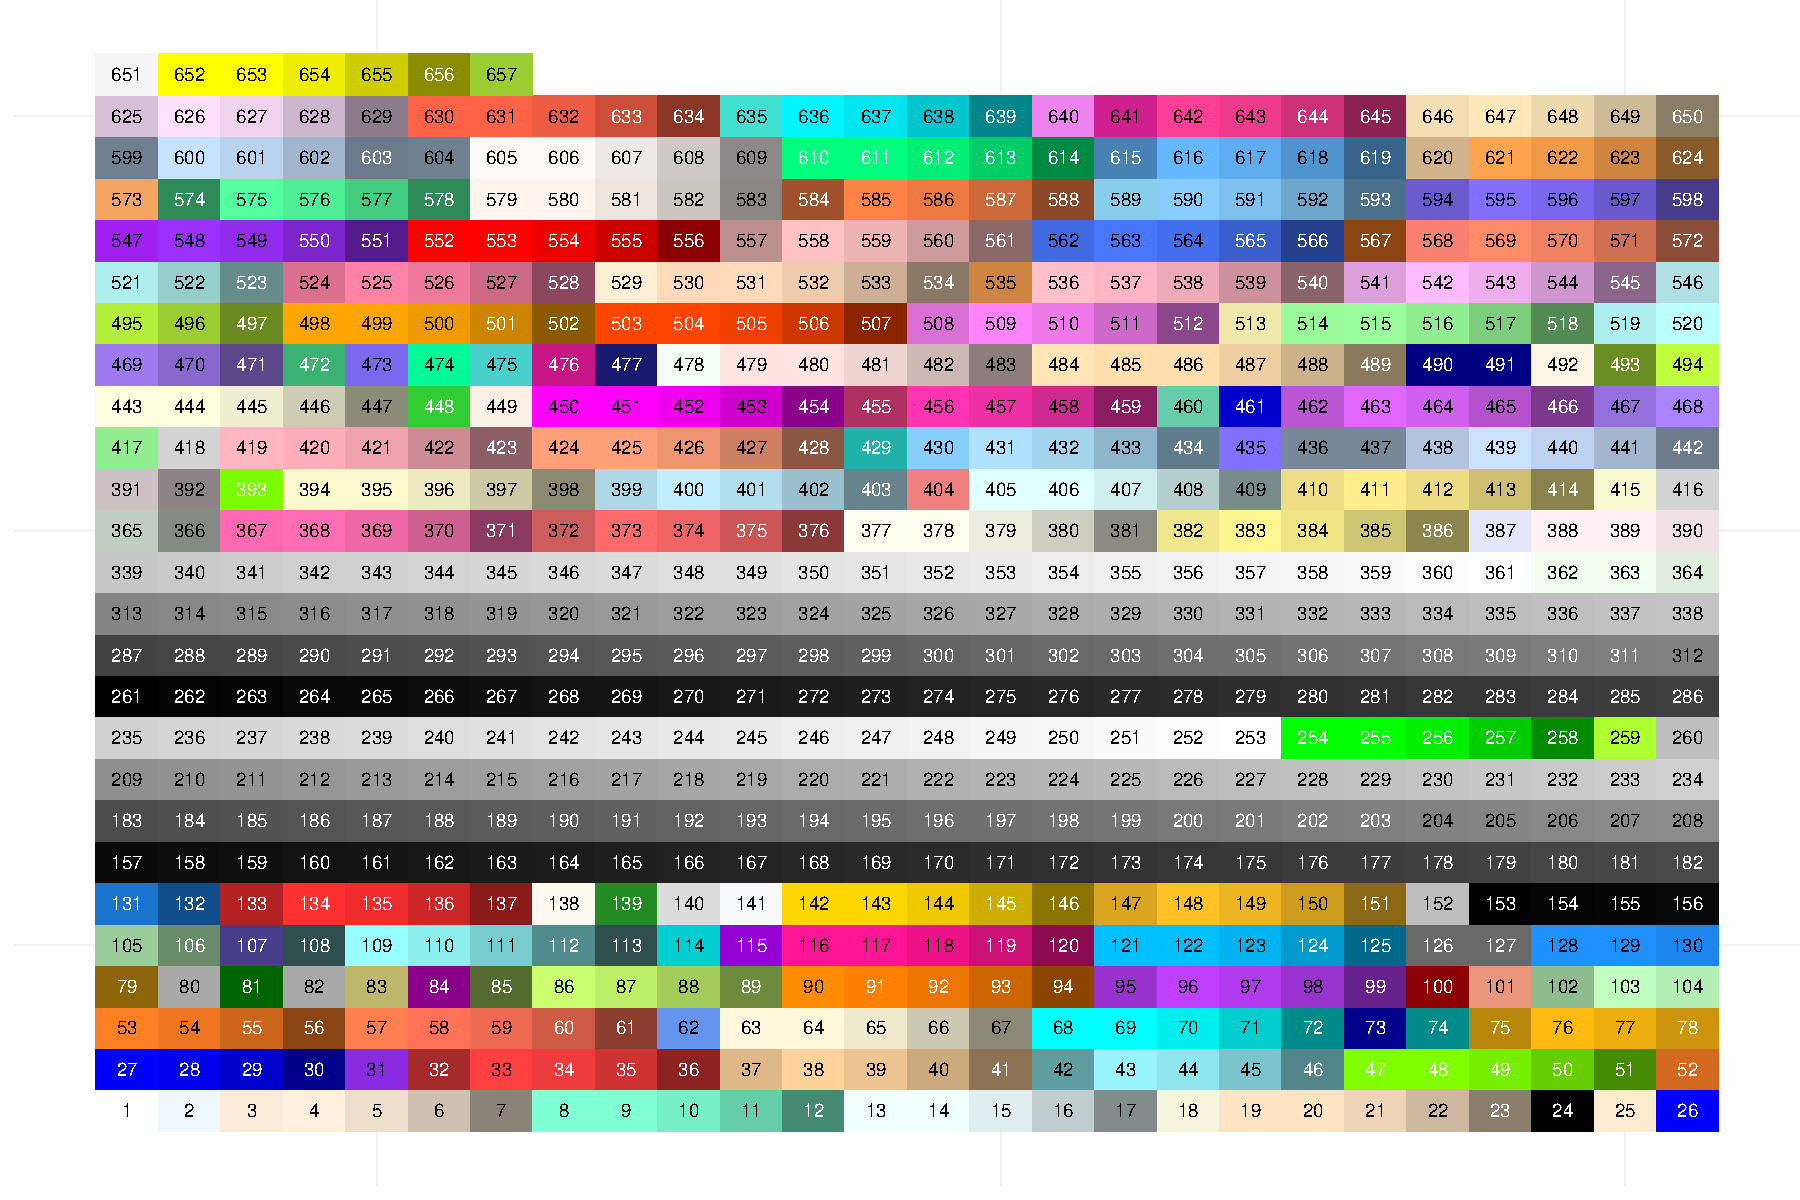
\includegraphics{Slides-colors}
\end{frame}





\section{likert Package}

\begin{frame}[containsverbatim,fragile]
	\frametitle{likert Package}
	The \texttt{likert} package provides functions to analyze and visualize Likert items. The graphics are created using \texttt{ggplot2}.
	
\begin{Schunk}
\begin{Sinput}
> require(devtools)
> install_github("likert","jbryer")
\end{Sinput}
\end{Schunk}

    The package includes a subset of the PISA data. Item 28 of the student questionnaire contains 11 items about student reading habits.
    
\begin{Schunk}
\begin{Sinput}
> require(likert)
> data(pisaitems)
> items28 = pisaitems[,substr(names(pisaitems), 1,5) == "ST24Q"]
\end{Sinput}
\end{Schunk}

\end{frame}

\begin{frame}[containsverbatim,fragile]
	\frametitle{Data Setup}
    First, rename the columns to the item stems.
    
\begin{Schunk}
\begin{Sinput}
> items28 <- rename(items28, c(
   			ST24Q01="I read only if I have to.",
   			ST24Q02="Reading is one of my favorite hobbies.",
   			ST24Q03="I like talking about books with other people.",
   			ST24Q04="I find it hard to finish books.",
   			ST24Q05="I feel happy if I receive a book as a present.",
   			ST24Q06="For me, reading is a waste of time.",
   			ST24Q07="I enjoy going to a bookstore or a library.",
   			ST24Q08="I read only to get information that I need.",
   			ST24Q09="I cannot sit still and read for more than a few minutes.",
   			ST24Q10="I like to express my opinions about books I have read.",
   			ST24Q11="I like to exchange books with my friends"))
\end{Sinput}
\end{Schunk}
\end{frame}


\begin{frame}[containsverbatim,fragile, shrink=20]
	\frametitle{Analyzing Likert Items}
    The \texttt{likert} function will analyze the items.
    
\begin{Schunk}
\begin{Sinput}
> l28 = likert(items28)
\end{Sinput}
\end{Schunk}
    
    And the \texttt{print} method will provide percentages of each category.
\begin{Schunk}
\begin{Sinput}
> print(l28)
\end{Sinput}
\begin{Soutput}
                                                       Item
1                                 I read only if I have to.
2                    Reading is one of my favorite hobbies.
3             I like talking about books with other people.
4                           I find it hard to finish books.
5            I feel happy if I receive a book as a present.
6                       For me, reading is a waste of time.
7                I enjoy going to a bookstore or a library.
8               I read only to get information that I need.
9  I cannot sit still and read for more than a few minutes.
10   I like to express my opinions about books I have read.
11                 I like to exchange books with my friends
   Strongly disagree Disagree Agree Strongly agree
1                 23       36    31           10.7
2                 20       36    32           11.4
3                 21       34    36            9.0
4                 25       40    27            8.1
5                 19       28    40           12.9
6                 42       41    11            6.1
7                 18       33    37           11.9
8                 15       35    36           13.8
9                 33       43    17            6.8
10                14       28    44           15.1
11                23       33    32           12.4
\end{Soutput}
\end{Schunk}
\end{frame}

\begin{frame}[containsverbatim,fragile,shrink=20]
	\frametitle{Likert SUmmary}
    The \texttt{summary} method will provide provide descriptive statistics.
    
\begin{Schunk}
\begin{Sinput}
> summary(l28)
\end{Sinput}
\begin{Soutput}
                                                       Item low high mean   sd
1                                 I read only if I have to.  59   41  2.3 0.94
2                    Reading is one of my favorite hobbies.  57   43  2.3 0.93
3             I like talking about books with other people.  55   45  2.3 0.91
4                           I find it hard to finish books.  65   35  2.2 0.90
5            I feel happy if I receive a book as a present.  47   53  2.5 0.94
6                       For me, reading is a waste of time.  83   17  1.8 0.86
7                I enjoy going to a bookstore or a library.  51   49  2.4 0.92
8               I read only to get information that I need.  50   50  2.5 0.91
9  I cannot sit still and read for more than a few minutes.  76   24  2.0 0.88
10   I like to express my opinions about books I have read.  41   59  2.6 0.90
11                 I like to exchange books with my friends  56   44  2.3 0.96
\end{Soutput}
\end{Schunk}
\end{frame}

\begin{frame}[containsverbatim,fragile]
	\frametitle{Bar Plot}
    The \texttt{summary} method will provide provide descriptive statistics.
    
\begin{Schunk}
\begin{Sinput}
> print(plot(l28))
\end{Sinput}
\end{Schunk}
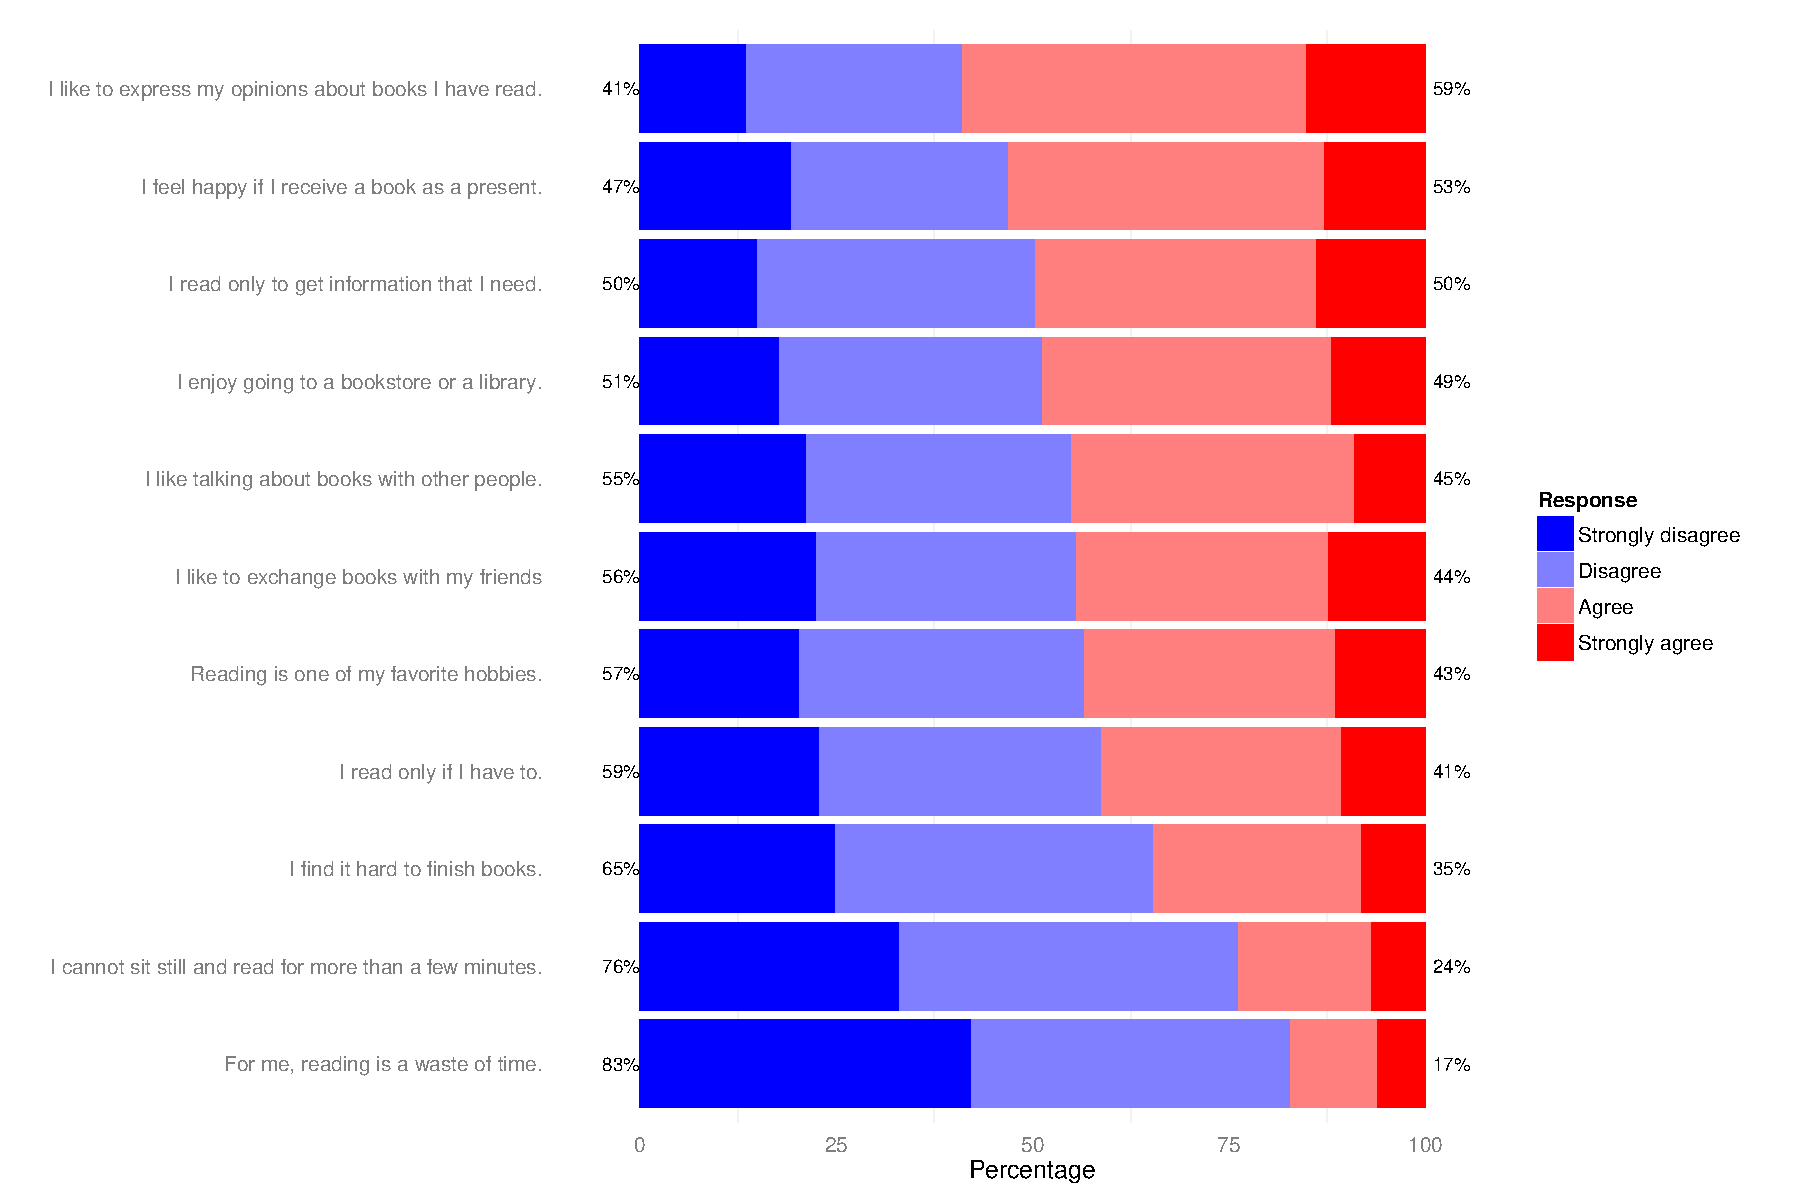
\includegraphics{Slides-likert-bar}
\end{frame}

\begin{frame}[containsverbatim,fragile]
	\frametitle{Bar Plot Centered}
    The \texttt{summary} method will provide provide descriptive statistics.
    
\begin{Schunk}
\begin{Sinput}
> print(plot(l28, centered=TRUE, low.color="#FF9900", high.color="#660066")
   )
\end{Sinput}
\end{Schunk}
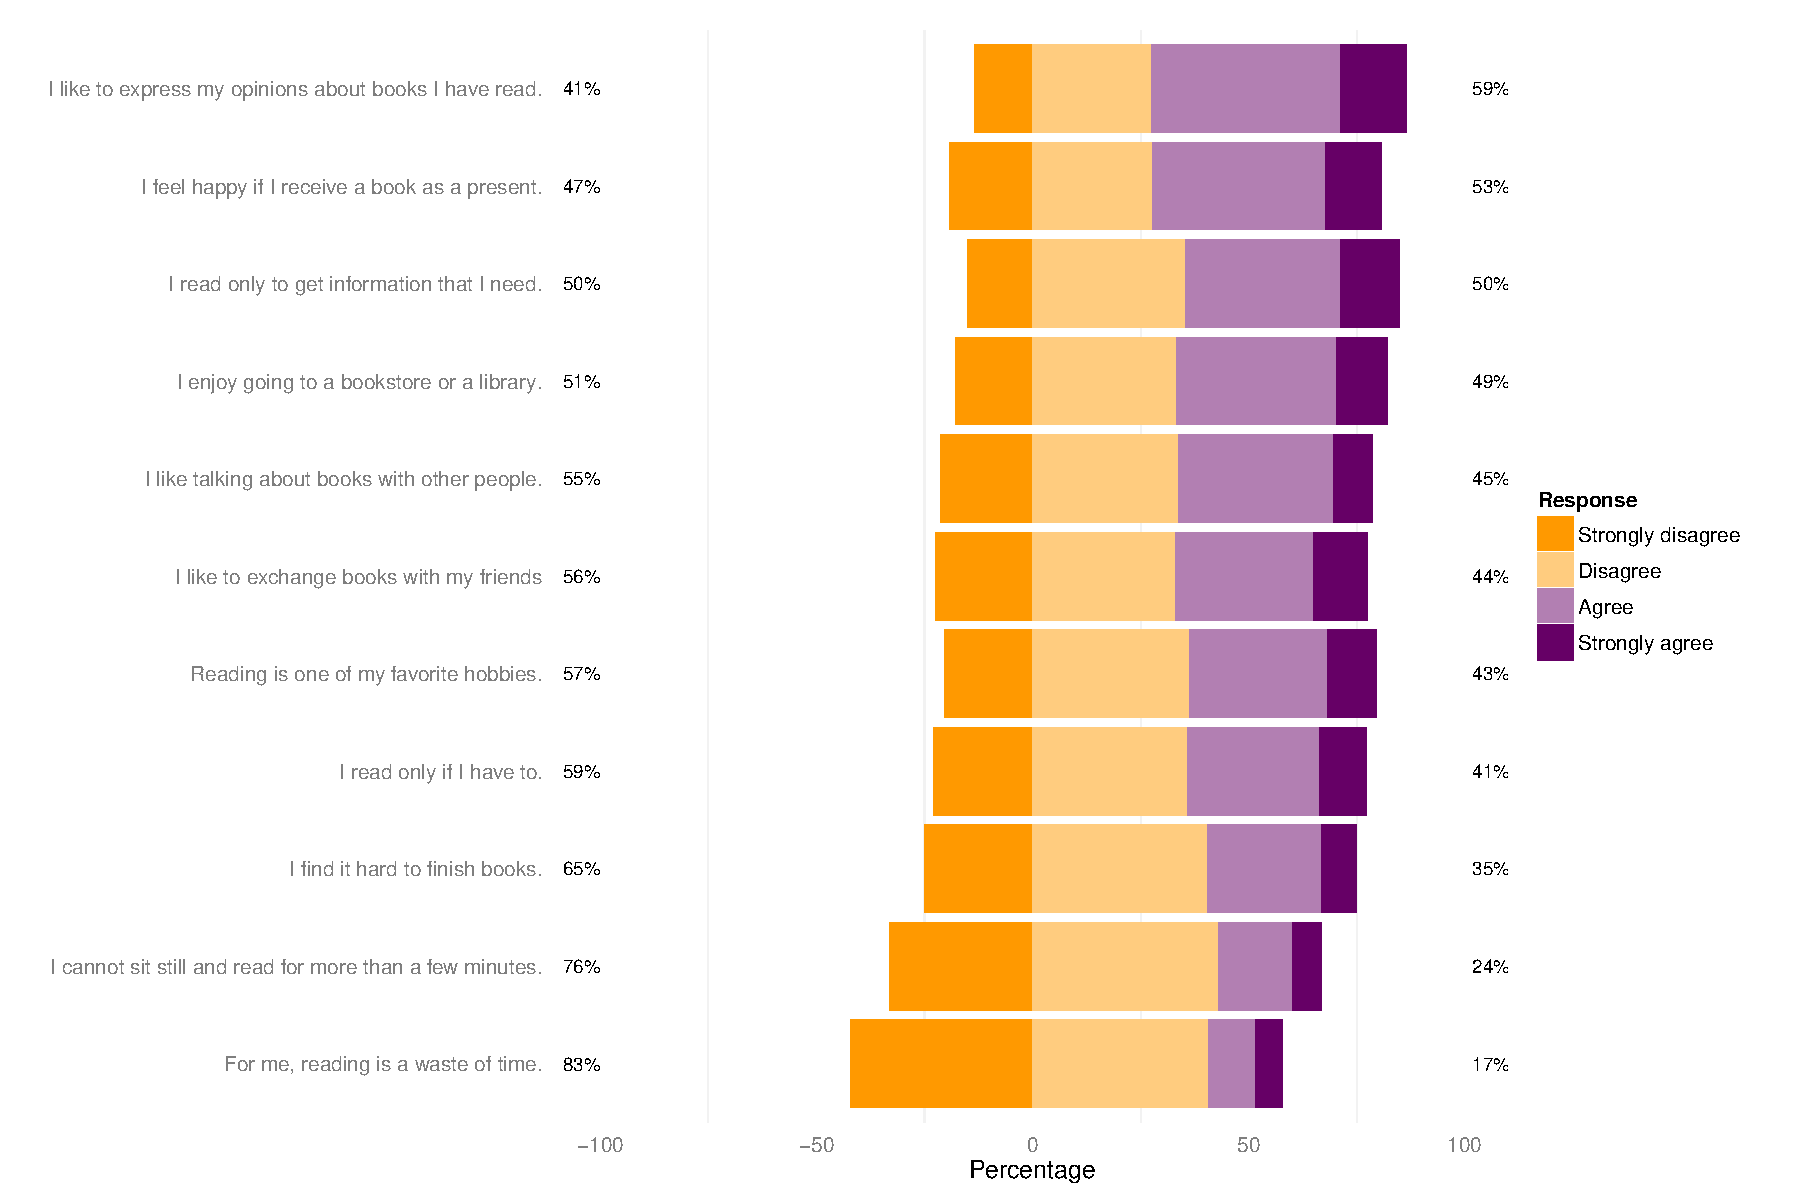
\includegraphics{Slides-likert-bar-centered}
\end{frame}

\begin{frame}[containsverbatim,fragile]
	\frametitle{Heat Map}
    The \texttt{summary} method will provide provide descriptive statistics.
    
\begin{Schunk}
\begin{Sinput}
> print(plot(l28, type="heat"))
\end{Sinput}
\end{Schunk}
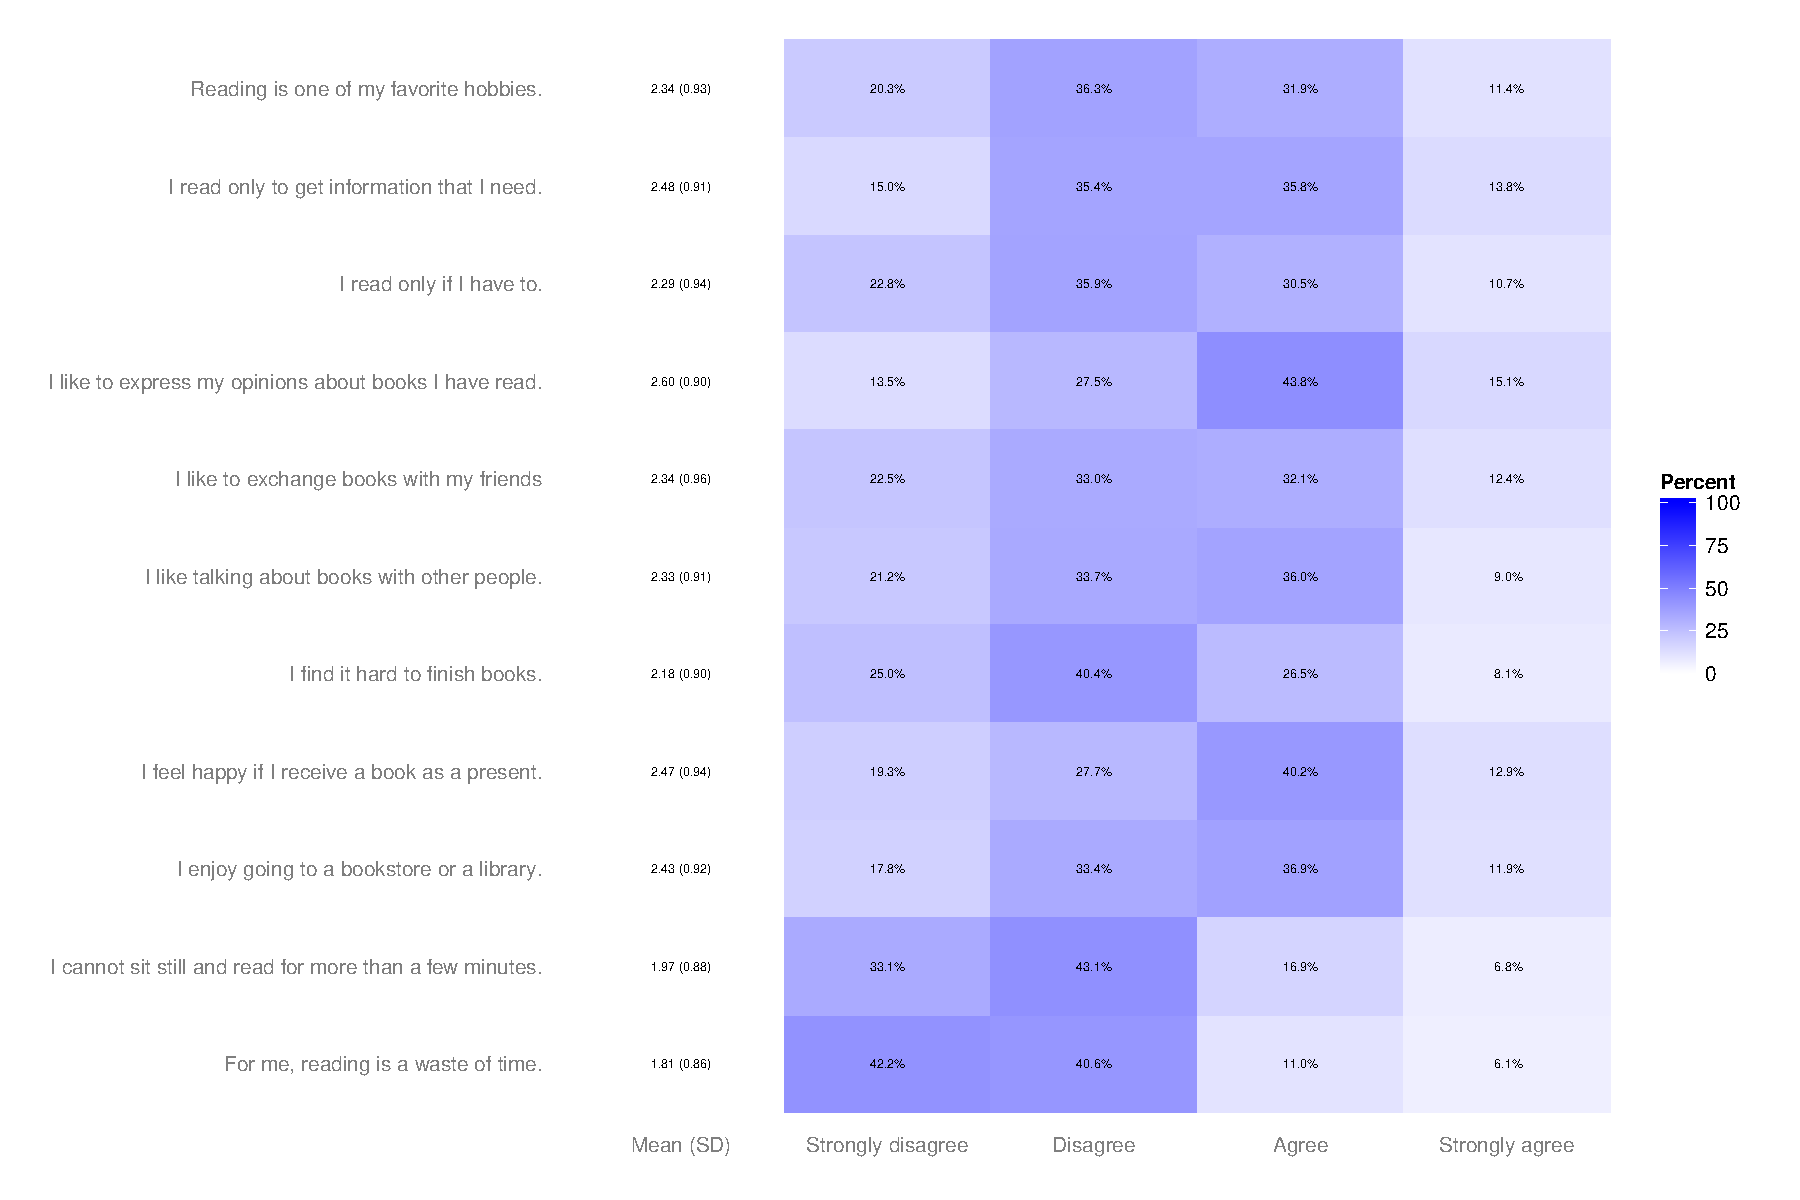
\includegraphics{Slides-likert-heat}
\end{frame}


%\begin{frame}[c]
%	\LARGE{Thank You}\\
%	\normalsize
%	Jason Bryer (jason@bryer.org)\\
%	\url{http://jbryer.github.com}
%\end{frame}

\end{document}
